\chapter{Experimental Design} \label{ch:Exp_Design}

\section{Testing Considerations}

\begin{wrapfigure}{r}{0.4\textwidth}
  \centering
    \includegraphics[width=0.4\textwidth]{whole_cart}
  \caption[Mobile Test Stand]{The mobile test stand, fully assembled. The aluminum rail holds the sensor mount 1~meter above the floor and is marked with an adhesive metric ruler for measuring camera displacement during PTAM initialization.}
  \label{fig:whole_cart}
\end{wrapfigure}

Before venturing further, we now summarize the goals of the UKF framework described previously, paying particular attention to the needs of unmanned aircraft system (UAS) operations. This ROS package was designed with the intent of producing estimates of the state of a rotorcraft UAV in real time. Thus, the experiments testing the system's efficacy compare the filter's estimates to the ground truth as measured by Vicon. Vicon, like many commercially available motion capture systems, works by using a number of infrared cameras (usually 8--12) to track the positions of retroreflector balls in the cameras' field of view. Each camera is outfitted with infrared LED\footnote{``Light-emitting diode,'' \url{https://en.wikipedia.org/wiki/Light-emitting_diode}} bulbs which illuminate the area with infrared light. The retroreflector balls reflect this infrared light back to the cameras, allowing the balls to be tracked as they move. Sets of these retroreflectors can be grouped together in software to represent rigid objects, allowing the Vicon system to track not only the position of an object, but its orientation as well.

\begin{figure}[t]
    \centering
    \begin{subfigure}[t]{0.5\textwidth}
        \centering
        \includegraphics[width=0.8\textwidth]{sensor_mount_top}
        \caption{Top view of sensor mount.}
    \end{subfigure}%
    ~ 
    \begin{subfigure}[t]{0.5\textwidth}
        \centering
        \includegraphics[width=0.8\textwidth]{sensor_mount_bottom}
        \caption{Bottom view of sensor mount.}
    \end{subfigure}
    \caption[3D-printed Sensor Mount]{The 3D-printed sensor mount. In (a), the Phidgets IMU is on the left and the mvBlueFOX camera is on the right. In (b), the linear braking handle and camera lens are visible.}
    \label{fig:sensor_mount}
\end{figure}

\begin{wrapfigure}{r}{0.4\textwidth}
  \centering
    \includegraphics[width=0.4\textwidth]{cart_at_AI}
  \caption[Testing Environment]{The mobile test stand in the testing environment. The area shown is part of a larger motion capture facility. The floor is covered with rubber tiles, many of which bear April tags and QR codes for visual geometry.}
  \label{fig:cart_at_AI}
\end{wrapfigure}

The UKF framework depends upon two sensors: a global-shutter monocular camera and an IMU. The IMU used in this experiment contains a 3-axis accelerometer and 3-axis gyroscope. To simulate both sensors moving through the scene in a manner reminiscent of hovering rotorcraft flight, a rolling test stand was constructed to carry the sensors safely throughout a large motion capture environment. Mounting the sensor suite (Figure~\ref{fig:sensor_mount}) on a large, steady, level platform (Figure~\ref{fig:whole_cart}) allows for a high degree of control over the accelerations and angular velocities felt by the IMU, as well as the motion captured by the ventral camera. In order to validate the UKF framework's effectiveness under ideal conditions, a modern laptop computer containing an Intel i7 processor with 16~GB of RAM\footnote{``Random-access memory,'' \url{https://en.wikipedia.org/wiki/Random-access_memory}} was used for all computations. The floor of the motion capture environment (Figure~\ref{fig:cart_at_AI}) was covered with rubber tiles and strewn with a mixture of April tags and modified Quick Response\footnote{\url{https://en.wikipedia.org/wiki/QR_code}} (QR) codes in order to provide sufficient visual features for PTAM to track.

\subsection{PTAM Anomalies}

The experiments chosen to test the system's effectiveness were influenced largely by the known capabilities and limitations of the ROS PTAM implementation\footnote{From here on, ``PTAM'' refers to the particular ROS implementation of PTAM used in the experiments, not to the algorithm in general.}. In previous exploratory experiments\footnote{Performed both by the author and by various other parties at NASA Langley, where the experiments described here took place.}, PTAM was frequently shown to lose tracking\footnote{``Tracking'' here refers to current pose knowledge.} during large rotations. PTAM is particularly susceptible to losing tracking during \textit{pure} rotations, in which the camera rotates in place without translational motion. Worse, whenever PTAM undergoes a rotation, it interprets this as an arc-like motion, regardless of whether any translation took place.

\begin{wrapfigure}{r}{0.4\textwidth}
    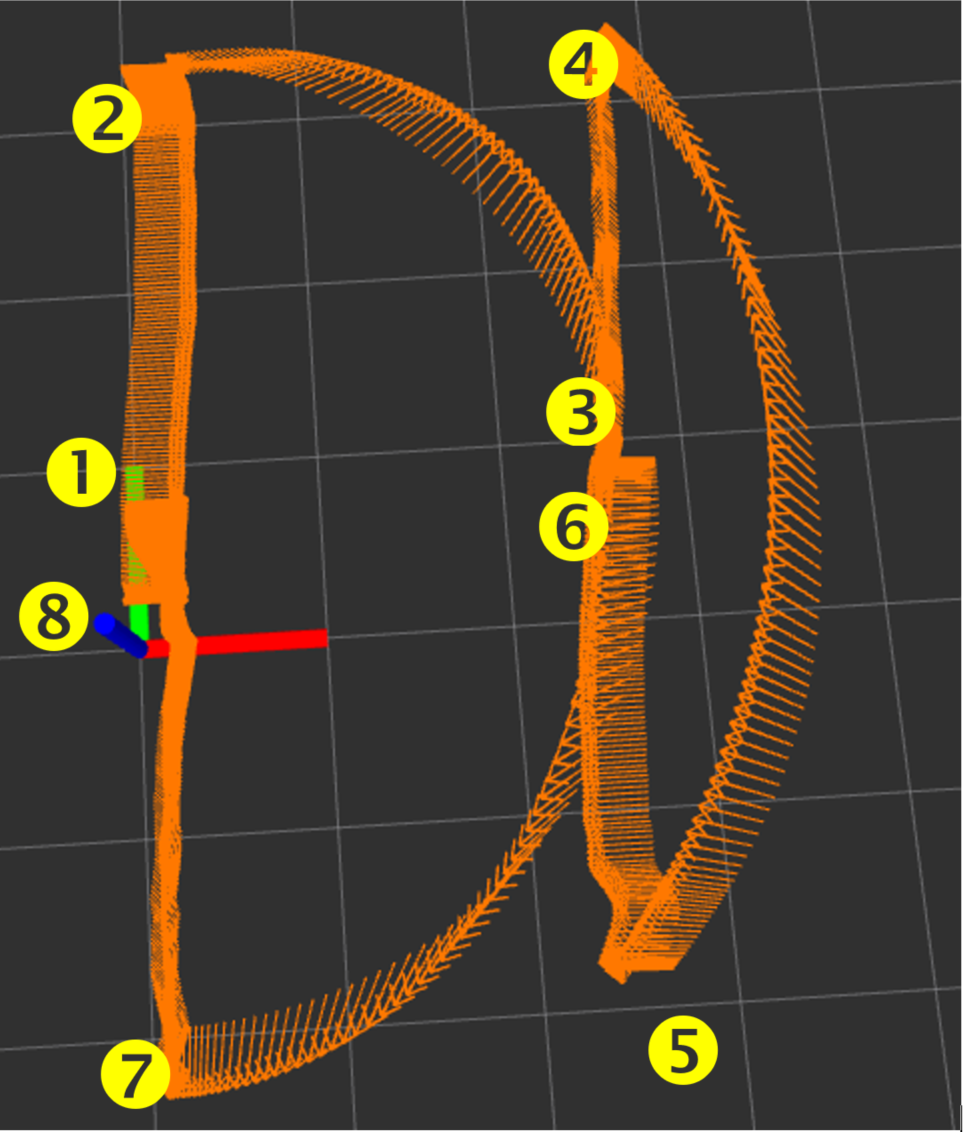
\includegraphics[width=0.4\textwidth]{rot_bug_rviz}
  \caption[Rviz Visualization of Rotational Distortion]{An Rviz visualization of PTAM's rotation defect. This image was created by moving the cart in a 3~m square pattern, turning 90\textdegree\ CCW at each corner.}
  \label{fig:rot_bug_rviz}
\end{wrapfigure}

Figure~\ref{fig:rot_bug_rviz} shows PTAM's susceptibility to losing tracking during rotation. This Rviz\footnote{A ROS visualization utility. \url{http://wiki.ros.org/rviz}} visualization was produced by moving the cart in a square trajectory and turning the cart by 90 degrees at each corner. In the figure, the vehicle's trajectory is traced out by a series of orange arrows representing the vehicle's $x$-axis. The vehicle started at the origin (Point~1), then moved forward (in the $+y$ direction) in a straight line to Point~2. At Point~2, the cart was rotated counterclockwise in place by 90 degrees, producing the arc between Points~2 and 3. At this point, the cart was pointed in the $-x$ direction. As the figure shows, this arc extends \textit{opposite} the camera's true direction of travel. After rotating 90 degrees, the vehicle moved in a straight line in the $-x$ direction (Point~3 to Point~4), then rotated again by 90 degrees such that the cart was pointed in the $-y$ direction (Point~4 to 5). Again, the arc goes backward from the actual direction of travel, but this time its length is much greater. This was caused by rotating the vehicle at a higher speed than during the first turn, meaning that this rotation defect is velocity-dependent. From Point~5, the vehicle moves in the $-y$ direction to Point~6, rotates 90 degrees counterclockwise (Point~6 to 7), and then moves in a straight line back to a point near the origin (Point~8).

The trajectory plotted in Figure~\ref{fig:rot_bug_rviz} is vastly distorted. A trusting observer might surmise from the image that the vehicle moved in a pattern resembling two uppercase D's, as opposed to the square pattern traced out in reality. This rotation-translation defect in the ROS PTAM implementation is pervasive and prevents PTAM from being of any real use during rotation. For this reason, the experiments detailed in the next section were carefully performed without rotating the mobile test stand.

\begin{wrapfigure}{l}{0.4\textwidth}
  \centering
    \includegraphics[width=0.4\textwidth]{sensor_mount_vicon}
  \caption[Sensor Mount Instrumented with Retroreflectors]{Close-up view of the sensor mount instrumented with retroreflector balls.}
  \label{fig:sensor_mount_vicon}
\end{wrapfigure}

In other preliminary experiments, anomalous behavior was discovered in PTAM's $z$-position output. Over long translations, the vehicle's estimated altitude could be seen rising erroneously the farther the vehicle moved from the origin. Figure~\ref{fig:bowl-shaped_world} shows a trajectory traced out by moving the test stand several meters to the left and right of the origin in a straight line. In profile, the visualized trajectory is clearly curved. This ``bowl-shaped'' trajectory would seem to arise from lens distortion not properly eliminated by PTAM. PTAM's calibration procedure was repeated several times to try to solve this problem but the distortion persisted. The mvBlueFOX camera has a wide-angle lens with a 150\textdegree\ field of view. During the calibration procedure, camera parameters were computed that, according to the ROS PTAM documentation, were well within acceptable limits for a wide-angle lens. Nevertheless, the aberrant measurements continued.

\begin{figure}[H]
  \centering
    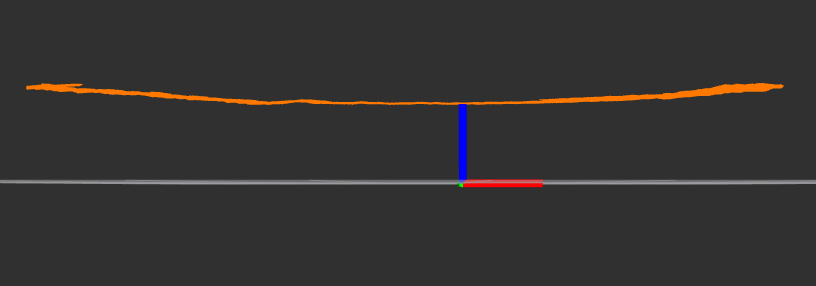
\includegraphics[width=\textwidth]{bowl-shaped_world}
  \caption[Rviz Visualization of Translational (Lens) Distortion]{An Rviz visualization of the ``bowl-shaped'' world seen by PTAM during a long translational motion. This image was created by translating the mobile test stand 3--4~meters in the $+x$ direction and then translating back 4--5~meters past the origin in the $-x$ direction.}
  \label{fig:bowl-shaped_world}
\end{figure}

\section{Experimental Procedures}

\begin{wrapfigure}{r}{0.4\textwidth}
  \centering
    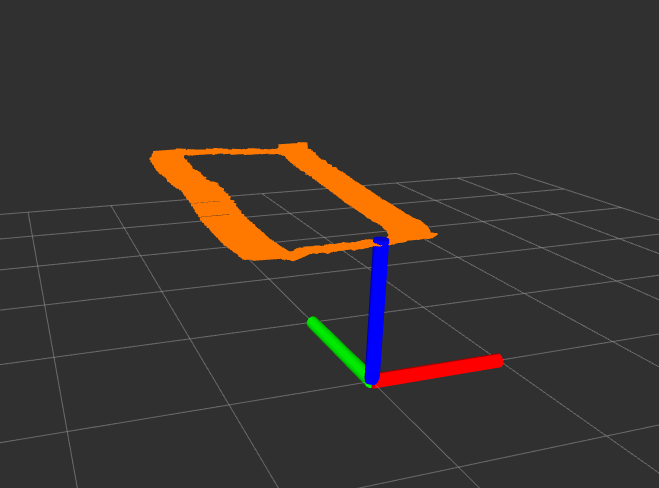
\includegraphics[width=0.4\textwidth]{good_box_5_cropped}
  \caption[Rviz Visualization of a Box Pattern Trajectory]{An Rviz visualization of a box pattern trajectory.}
  \label{fig:good_box}
\end{wrapfigure}

Two experiments were designed to characterize the UKF framework's effectiveness in various regimes of motion. The first experiment was a ``long walk'' in which the mobile test stand was translated in a straight line for several meters along the $y$-axis. This test was designed to characterize the effect of lens distortion on PTAM's $z$-position output, as discussed previously. In the second experiment, the mobile test stand was moved in a rectangular ``box'' pattern (Figure~\ref{fig:good_box}) to determine the system's efficacy in planar motions indicative of hovering flight. Both experiments took place on a level floor to capture more accurately any $z$-directional distortion. Because of the rotation-translation coupling defect found in PTAM, the mobile test stand was moved carefully in each experiment such that it would undergo minimal rotation and thus accurately capture translational motion.

Prior to each trial of each experiment, PTAM was initialized according to the procedure outlined in the documentation. To initialize the algorithm, the camera was placed parallel to the floor at a distance of one meter and then perturbed by 10\% of the distance to the floor (that is, 10~cm). This perturbation tells PTAM its distance to the planar surface in view and thus initializes the map. This initialization procedure was performed by releasing the linear bearing brake on the sensor mount and sliding the mount along the aluminum rail, using the attached adhesive ruler to perturb the camera by exactly 10~cm. After perturbing the camera, the brake was tightened, and the data recording began.

For each long walk trial, the mobile test stand was moved forward in the $+y$ direction by 4--6~meters, being carefully to perturb the stand as little as possible along the $x$-axis. Some amount of lateral instability was unavoidable, however, due to the nature of the floor on which these trials were performed. The rubber tiles covering the floor of the testing area concealed a number of power cables for nearby computers, presenting small ``bumps'' over which the test stand had to pass. These bumps caused uneven left--right perturbations to the test stand, which, though minor in magnitude, proved to be noticeable in post processing (see Chapter~\ref{ch:Exp_Results}). When the test stand had been pushed to the end of the long walk segment, it was then pulled backward in the $-y$ direction until it had approximately returned to the origin.

For the box pattern trials, the mobile test stand was first moved forward in the $+y$ direction by 2.5 to 3~meters. Then, without rotating, the test stand was pushed leftward in the $-x$ direction by approximately 1~meter. The test stand was then pulled backward in the $-y$ direction by 2.5 to 3~meters, returning approximately to $y = 0$. Finally, the test stand was pushed to the right ($+x$) to return to the origin.

\clearpage
\section{Materials}
\subsection{Computation and Sensing}
\begin{enumerate}
\item One (1) MatrixVision mvBlueFOX-MLC Camera\footnote{\url{https://www.matrix-vision.com/USB2.0-single-board-camera-mvbluefox-mlc.html}}
\item One (1) 1044\_0 PhidgetSpatial Precision 3/3/3 High Resolution IMU\footnote{\url{http://www.phidgets.com/products.php?product_id=1044}}
\item One (1) Hewlett-Packard Spectre x360 Convertible Laptop 13-ac076nr\footnote{\url{http://store.hp.com/us/en/pdp/hp-spectre-x360---13-ac076nr}}
\item Two (2) male Mini USB 2.0 to male USB Type A cables
\end{enumerate}
\subsection{Mobile Test Stand}
\begin{enumerate}
\item One (1) Oklahoma Sound PRC200 Premium Presentation Cart\footnote{\url{http://www.oklahomasound.com/products/product-category/single/?prod=9}}
\item One (1) 3D-printed Sensor Mount
\item Two (2) 4" C-Clamps
\item One (1) 1.2-meter 80/20\textsuperscript{\textregistered}~Inc.\ 1515 Rail\footnote{\url{https://8020.net/1515.html}}
\item One (1) 15 Series ``L'' Handle Linear Bearing Brake Kit\footnote{\url{https://8020.net/6800.html}}
\item One (1) $\frac{5}{16}$-18 $\times$ 0.687" Black FBHSCS (Screw)\footnote{\url{https://8020.net/shop/3320.html}}
\item Two (2) Slide-In Economy T-Nuts\footnote{Also available at \url{https://8020.net/shop/3320.html}}
\item Three (3) 1" Vicon Infrared Retroreflector Balls
\item Two (2) $\frac{1}{2}$" Vicon Infrared Retroreflector Balls
\item One (1) 0.7-meter Length of $\frac{1}{8}$"-thick Carbon Fiber Tube
\end{enumerate}
\pagebreak